\section{Results}
\label{sec:results}

Our analysis reveals a systematic divergence between the default spatial narratives generated by LLMs and those generated with human-centric prompting. The statistical summary of our findings is presented in \tabref{tab:results}.

\begin{table}[t]
\centering
\caption{Linguistic feature comparison across models and prompting conditions. Best results (highest variance/entropy) in \textbf{bold}.}
\label{tab:results}
\resizebox{\textwidth}{!}{%
\begin{tabular}{lcccc}
\toprule
\textbf{Condition} & \textbf{Prep. Entropy (bits)} & \textbf{Avg. Length (words)} & \textbf{Length Var.} & \textbf{Unique Preps} \\
\midrule
\gptom (\standardprompt) & 3.77 & 5.87 & 5.27 & 24 \\
\gpto (\standardprompt) & 3.41 & 7.64 & 5.91 & 22 \\
\midrule
\gptom (\humanprompt) & \textbf{3.84} & \textbf{10.85} & \textbf{8.98} & \textbf{33} \\
\bottomrule
\end{tabular}
}
\end{table}

\para{Vocabulary Bias (H1)}
We hypothesize that LLMs in their standard configuration would exhibit a restricted spatial vocabulary. Our results support this: \gpto (\standardprompt) exhibited the lowest \prepentropy at 3.41 bits, using only 22 unique prepositions across the entire dataset. This indicates a strong preference for a limited set of topological descriptors (e.g., "into", "through", "past") without stylistic variation. In contrast, the \humanprompt condition increased unique preposition usage to 33, representing a 50\% increase in vocabulary diversity (\figref{fig:entropy}).

\para{Structural Rigidity (H2)}
Default models produced highly uniform sentence structures. \gptom (\standardprompt) showed a \sentvar of only 5.27, with an average sentence length of 5.87 words. This reflects a rigid "Subject-Verb-Direction" pattern (e.g., "I walked into the kitchen."). When prompted to be human-like, the variance nearly doubled to 8.98, and the average sentence length increased to 10.85 words (\figref{fig:variance}). This change suggests that the default "robotic" tone is a choice induced by the model's standard operating mode rather than a lack of linguistic capability.

\para{Syntactic Patterns}
The Part-of-Speech (POS) bigram analysis further identifies this structural rigidity.
\begin{itemize}[leftmargin=*,itemsep=0pt,topsep=0pt]
    \item {\bf Standard Conditions}: Top bigrams across both \gptom and \gpto included \texttt{(ADP, DET)}, \texttt{(PRON, VERB)}, and \texttt{(NOUN, PUNCT)}. This confirms a predictable, topological mapping structure.
    \item {\bf Human Prompt Condition}: While sharing common bigrams, this condition uniquely introduced \texttt{(ADJ, NOUN)} into the top 5 structural bigrams. This confirms our third hypothesis (H3) that default LLM narratives prioritize topological relations over sensory/experiential descriptions, which require adjectives to ground the space.
\end{itemize}

\begin{figure}[t]
    \centering
    \begin{subfigure}[b]{0.45\textwidth}
        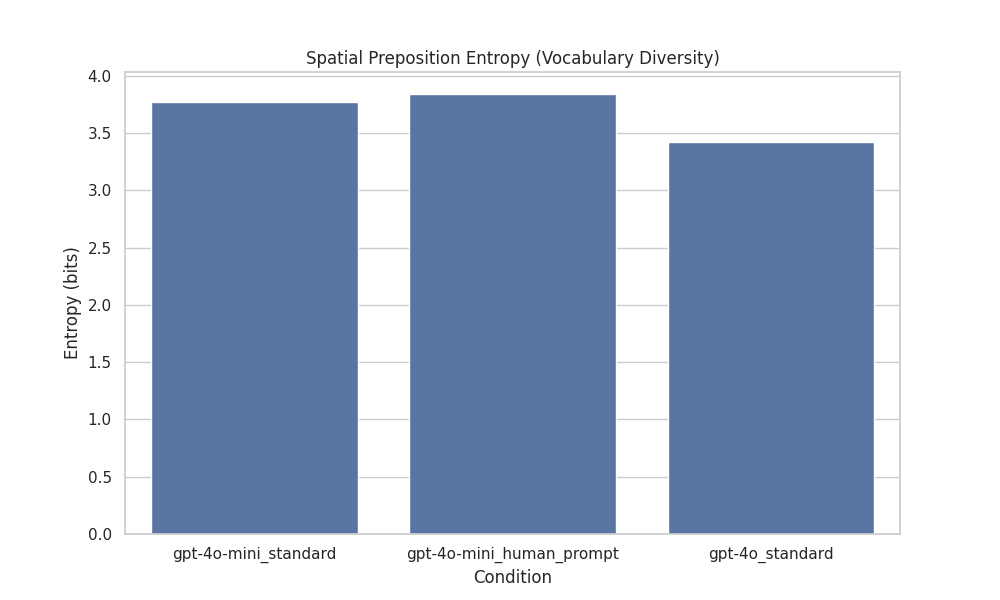
\includegraphics[width=\textwidth]{figures/prep_entropy.png}
        \caption{Spatial Preposition Entropy}
        \label{fig:entropy}
    \end{subfigure}
    \hfill
    \begin{subfigure}[b]{0.45\textwidth}
        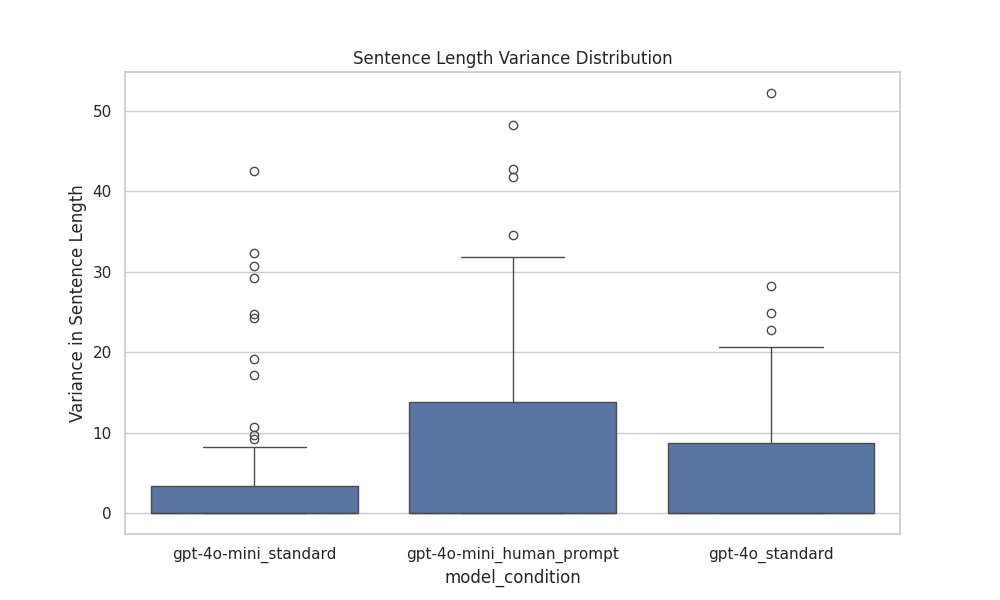
\includegraphics[width=\textwidth]{figures/sent_variance.png}
        \caption{Sentence Length Variance}
        \label{fig:variance}
    \end{subfigure}
    \caption{Linguistic variance analysis. (a) shows the dip in vocabulary diversity for standard \gpto. (b) shows the significant increase in structural variance when models are prompted to be "human-like."}
\end{figure}
